\documentclass[../ClipsManualeUtente.tex]{subfiles}

\begin{document}
\section{Per iniziare}
	Per iniziare ad utilizzare subito l'applicazione:
	\begin{enumerate}
		\item attiva il \textbf{bluetooth};
		\item attiva una \textbf{connessione dati} oppure una \textbf{connessione Wi-fi} e assicurati che lo smartphone sia connesso ad Internet;
		\item avvia l'applicazione selezionando l'icona %includegraphics[scale=0.1]{img/LogoApp};
		\item assicurati di essere in un \textbf{edifico supportato} dall'applicazione. Per assicurarsi di ciò basta accertarsi che dalla schermata principale dell'applicazione siano visibili le informazioni dell'edificio;
		
		\begin{figure} [h]
			\centering
			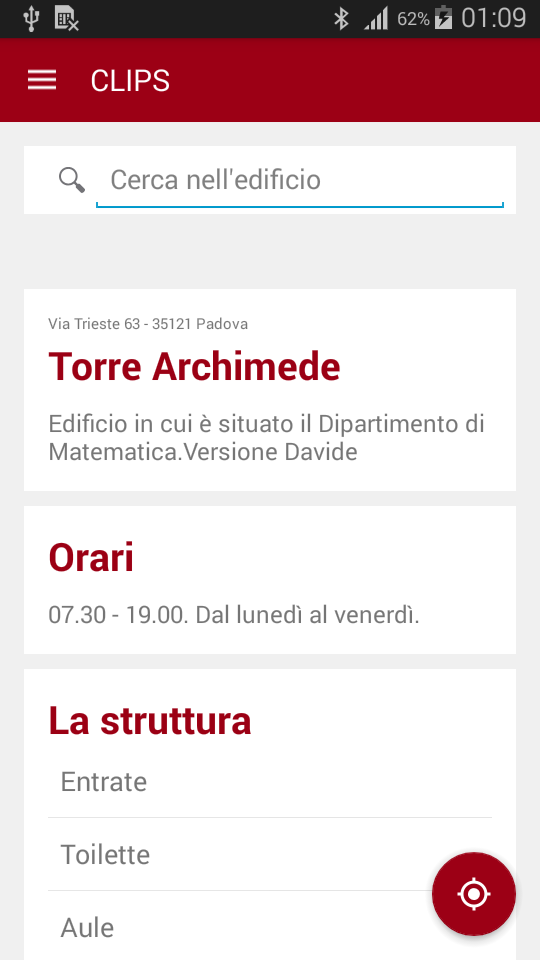
\includegraphics[scale=0.2]{img/HomeApp}
			\caption{Schermata principale dell'applicazione che riporta le informazioni dell'edificio in cui ci si trova}
			\label{fig:HomeApp}
		\end{figure}
		
		\item nella schermata principale, se l'edificio, è stato identificato potrai trovare:
		\begin{itemize}
			\item informazioni relative all'edificio: nome e indirizzo;
			\item orari di apertura e chiusura dell'edificio;
			\item una lista di categorie che raccolgono tutte le possibili aree d'interesse da raggiungere;
		\end{itemize}
		\item dalla lista sotto: \textit{`La Struttura'} seleziona la categoria di tuo interesse;
		
		\begin{figure} [h]
			\centering
			%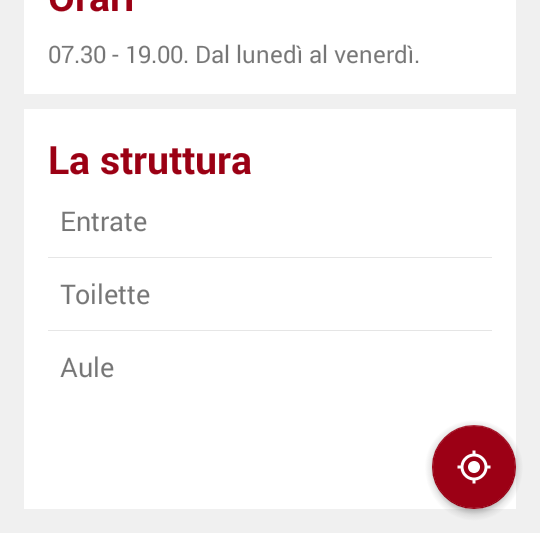
\includegraphics[scale=0.2]{img/CategoriePoi}
			\caption{Lista di categorie delle possibili destinazioni}
			\label{fig:CategoriePoi}
		\end{figure}	
		
		\newpage
		\item seleziona l'area d'interesse che vuoi raggiungere;
		
		\begin{figure} [h]
			\centering
			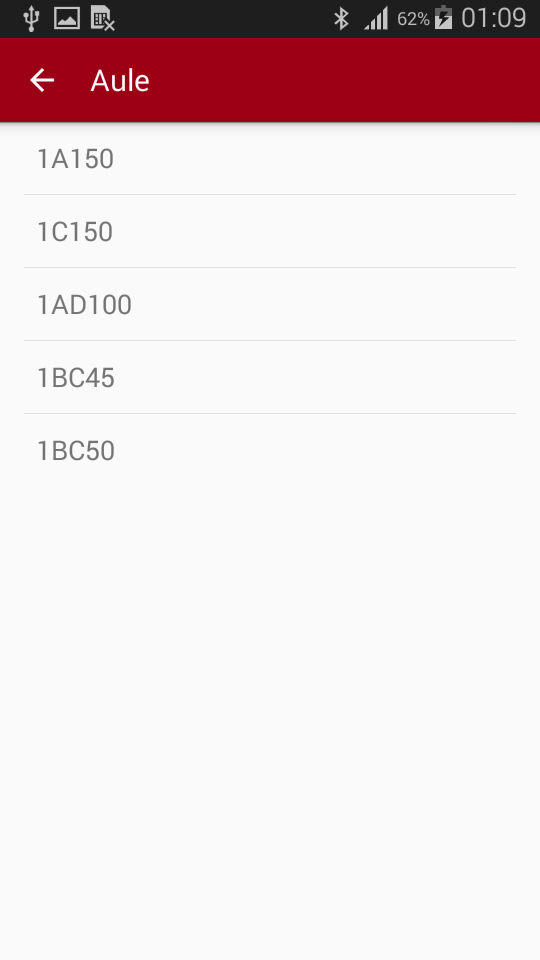
\includegraphics[scale=0.2]{img/ListaPoi}
			\caption{Lista delle possibili destinazioni della categoria \textit{`Aule'}}
			\label{fig:ListaPoi}
		\end{figure}				
		
		\item segui le indicazioni mostrate per raggiungere l'area scelta precedentemente.
		
		\begin{figure} [h]
			\centering
			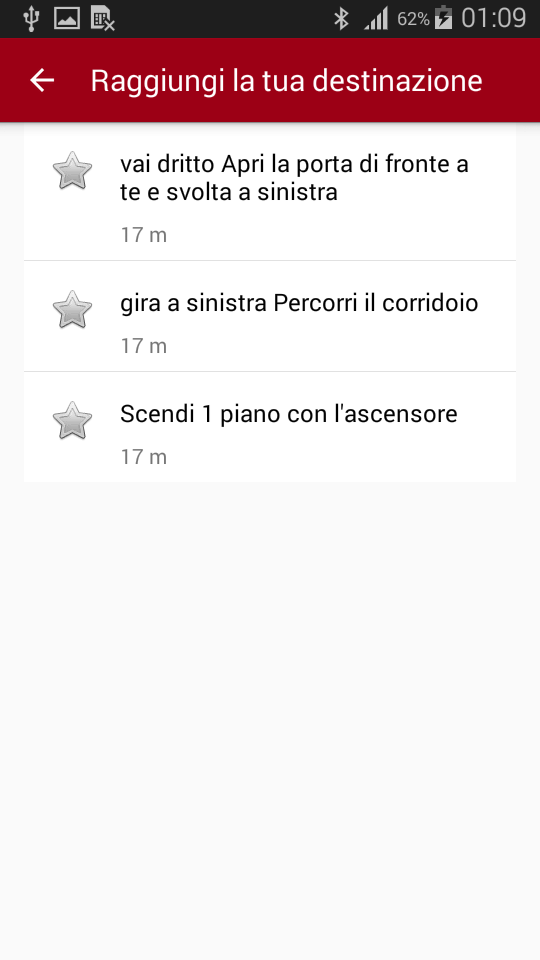
\includegraphics[scale=0.2]{img/ListaIstruzioni}
			\caption{Lista di istruzioni da seguire per raggiungere la destinazione scelta}
			\label{fig:ListaIstruzioni}
		\end{figure}	
		
	\end{enumerate}

\end{document}